% Ao menos uma linguagem (brazil ou english) deveria sempre ser fornecida
\documentclass{beamer}

\mode<presentation> {

% The Beamer class comes with a number of default slide themes
% which change the colors and layouts of slides. Below this is a list
% of all the themes, uncomment each in turn to see what they look like.

%\usetheme{default}
%\usetheme{AnnArbor}
%\usetheme{Antibes}
%\usetheme{Bergen}
%\usetheme{Berkeley}
%\usetheme{Berlin}
%\usetheme{Boadilla}
%\usetheme{CambridgeUS}
%\usetheme{Copenhagen}
%\usetheme{Darmstadt}
%\usetheme{Dresden}
%\usetheme{Frankfurt}
%\usetheme{Goettingen}
%\usetheme{Hannover}
%\usetheme{Ilmenau}
%\usetheme{JuanLesPins}
%\usetheme{Luebeck}
\usetheme{Madrid}
%\usetheme{Malmoe}
%\usetheme{Marburg}
%\usetheme{Montpellier}
%\usetheme{PaloAlto}
%\usetheme{Pittsburgh}
%\usetheme{Rochester}
%\usetheme{Singapore}
%\usetheme{Szeged}
%\usetheme{Warsaw}

% As well as themes, the Beamer class has a number of color themes
% for any slide theme. Uncomment each of these in turn to see how it
% changes the colors of your current slide theme.

%\usecolortheme{albatross}
%\usecolortheme{beaver}
%\usecolortheme{beetle}
%\usecolortheme{crane}
%\usecolortheme{dolphin}
%\usecolortheme{dove}
%\usecolortheme{fly}
%\usecolortheme{lily}
%\usecolortheme{orchid}
%\usecolortheme{rose}
%\usecolortheme{seagull}
%\usecolortheme{seahorse}
%\usecolortheme{whale}
%\usecolortheme{wolverine}

\setbeamertemplate{navigation symbols}{} % Remove the navigation symbols from the bottom of all slides
}

\usepackage[brazilian]{babel}
\usepackage[utf8]{inputenc}
\usepackage{abntex2cite}
\usepackage[useregional]{datetime2}
\usepackage{graphicx}
\usepackage{subcaption}
\usepackage{xcolor}

\usepackage[acronym,nowarn]{glossaries}
\makeglossaries

\newcommand{\mydate}{\DTMdisplaydate{2020}{9}{29}{-1}}

\setbeamertemplate{bibliography entry title}{}
\setbeamertemplate{bibliography entry location}{}
\setbeamertemplate{bibliography entry note}{}

%%%%%%%%%%%%%%%%%%%%%%%%%%%%
% Metadados
%%%%%%%%%%%%%%%%%%%%%%%%%%%%
\title[Avaliação LWMPI no Nanvix]{Avaliação de Desempenho utilizando biblioteca
MPI sobre Infraestrutura de Comunicação de Baixo Nível no Nanvix}
\author[Uller, J. F.]{\large João Fellipe Uller}

\institute[UFSC]
{
Universidade Federal de Santa Catarina \\
Depto. de Informática e Estatística (INE) \\
\medskip
INE410129-41000025DO/ME (20201) - Computação Paralela \\
Prof. Dr. Márcio Bastos Castro \\
\medskip
\textit{joao.f.uller@grad.ufsc.br}
}

\date{\mydate}

%%%%%%%%%%%%%%%%%%%%%%%%%%%%
% Slides
%%%%%%%%%%%%%%%%%%%%%%%%%%%%

\begin{document}

% Title page
\begin{frame}
  \titlepage
\end{frame}

% Sumario
\begin{frame}{Sumário}
  \tableofcontents
\end{frame}

%%%%%%%%%%%%%%%%%%%%%%%%%%%%
% Motivação
%%%%%%%%%%%%%%%%%%%%%%%%%%%%

\section{Motivação}

  \subsection{Contexto}
    \begin{frame}{Contexto}
      \begin{itemize}
        \item Poder computacional vs Consumo energético
        \item Preocupação crescente com a eficiência energética
      \end{itemize}
    \end{frame}

  \subsection{\textit{Lightweight manycores}}
    \begin{frame}{\textit{Lightweight Manycores}}
      \begin{itemize}
        \item Milhares de núcleos de baixa potência num mesmo \textit{chip},
          agrupados em \textit{clusters}
        \begin{itemize}
          \item Alto grau de paralelismo entre \textit{threads}!
        \end{itemize}
        \item Comunicação baseada em \textit{Message Passing} através de uma
          \textit{Network-on-Chip} (NoC) de alta vazão
        \item Subsistemas de memória restritivos
      \end{itemize}
    \end{frame}

    %
    \begin{frame}{Desafios}
      \begin{itemize}
        \item Porte de aplicações é uma tarefa complexa
        \begin{itemize}
          \item Precisa-se levar em conta características arquiteturais
        \end{itemize}
        \item Necessidade de ambientes de desenvolvimento que equilibrem desempenho,
          portabilidade e programabilidade
        \begin{itemize}
          \item \textbf{Implementação de uma biblioteca de comunicação segundo o
            padrão \textit{Message Passing Interface} (MPI), compatível com as
            restrições de \textit{Lightweight Manycores}}
        \end{itemize}
      \end{itemize}
    \end{frame}

%%%%%%%%%%%%%%%%%%%%%%%%%%%%
% LWMPI
%%%%%%%%%%%%%%%%%%%%%%%%%%%%

\section{LWMPI}

  \subsection{Visão geral}
    \begin{frame}{LWMPI}
      \begin{itemize}
        \item \textit{\textbf{L}ight\textbf{w}eight \textbf{M}essage \textbf{P}assing \textbf{I}nterface}
        \item Biblioteca de comunicação compatível com o padrão MPI (versão 3.1)
        \begin{itemize}
          \item Implementação "\textit{from scratch}" para ser compatível com as
            restrições de \textit{lightweight manycores}
          \item Implementa um subconjunto das funções MPI
        \end{itemize}
        \item Desenvolvida sobre a infraestrutura de Comunicação entre Processos (IPC) do Nanvix
      \end{itemize}
    \end{frame}

  \subsection{Nanvix}
    \begin{frame}{Nanvix}
      \begin{itemize}
        \item Sistema operacional (SO) de código aberto, compatível com POSIX (\url{https://github.com/nanvix/})
        \item Sistema distribuído para arquiteturas \textit{manycore}
        \item Baseado em uma estrutura \textbf{\textit{multikernel}}
        \begin{itemize}
          \item Múltiplas instâncias de um \textit{microkernel} assimétrico
        \end{itemize}
      \end{itemize}

      \begin{figure}
        \centering
        \subcaptionbox{Nanvix \textit{Multikernel}}{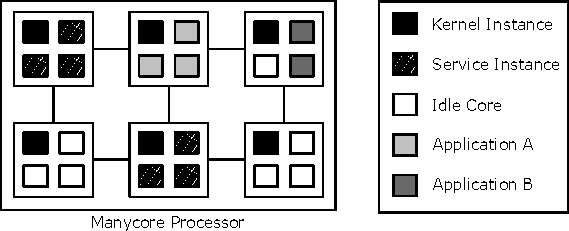
\includegraphics[width=0.65\linewidth]{images/multikernel.pdf}}
        \hspace{0.05\linewidth}
        \subcaptionbox{Nanvix \textit{Logo}}{
\includegraphics[width=0.25\linewidth]{images/nanvix.pdf}}
      \end{figure}
    \end{frame}

    %
    \begin{frame}{Abstrações Nanvix IPC}
      \begin{itemize}
        \item \textit{Mailbox}
        \item \textit{Portal}
        \item \textit{Sync}
      \end{itemize}
    \end{frame}

  \subsection{Estrutura}
    \begin{frame}{Estrutura LWMPI}
      \begin{figure}
        \centering
        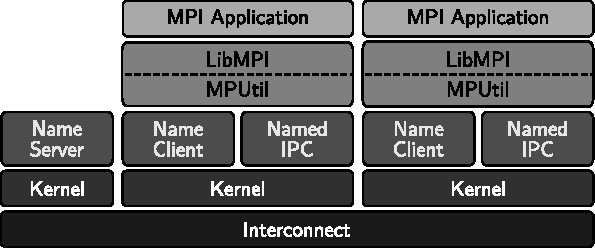
\includegraphics[width=0.9\linewidth]{images/libmpi.pdf}
        \caption{Estrutura LWMPI}
        \label{fig:lwmpi}
      \end{figure}
    \end{frame}

  \subsection{Suporte Atual}
    \begin{frame}{Suporte Atual}
      \begin{itemize}
        \item Comunicadores
        \item Grupos de comunicação
        \item Tratadores de erros
        \item \textit{Datatypes} padrão da linguagem C
        \item Comunicação ponto a ponto no modo síncrono (\texttt{MPI\_Send} e \texttt{MPI\_Recv})
      \end{itemize}
    \end{frame}

%%%%%%%%%%%%%%%%%%%%%%%%%%%%
% Proposta
%%%%%%%%%%%%%%%%%%%%%%%%%%%%

\section{Proposta}

  \subsection{Objetivo geral}
    \begin{frame}{Proposta}
      \begin{itemize}
        \item Porte de algumas aplicações utilizadas em \textit{benchmarking} para avaliar
          o desempenho da biblioteca desenvolvida (3 a 5 aplicações)
        \item Comparação com a infraestrutura de comunicação de baixo nível do Nanvix (Nanvix IPC)
        \begin{itemize}
          \item Forma de avaliar o \textit{overhead} introduzido pelo \textit{runtime}
        \end{itemize}
        \item Avaliação do tempo total, \textit{speedup}, além de técnicas de \textit{profiling}
          para avaliar possíveis gargalos e possibilidades de melhoria
      \end{itemize}
    \end{frame}

  \subsection{Metodologia}
    \begin{frame}{\textit{CAP Benchmarks}}
      \begin{itemize}
        \item Suite de \textit{benchmarking} utilizada para medir o desempenho
          de \textit{lightweight manycores}
        \item Caracterizado por sete aplicações que empregam diferentes padrões de
          computação e de paralelismo para avaliar um conjunto maior de características
        \begin{itemize}
          \item \textit{Features from Accelerated Segment Test (FAST)}
          \item \textbf{\textit{Friendly Numbers (FN)}}
          \item \textbf{\textit{Gaussian Filter (GF)}}
          \item \textit{Integer Sort (IS)}
          \item \textbf{\textit{K-Means (KM)}}
          \item \textit{LU Factorization (LU)}
          \item \textit{Traveling-Salesman Problem (TSP)}
        \end{itemize}
        \item Cenários variando de 1 a 15 \textit{workers}, além do processo líder
      \end{itemize}
    \end{frame}

  \subsection{Arquitetura alvo}
    \begin{frame}{Kalray MPPA-256}
      \begin{itemize}
        \item 16 \textit{Compute Clusters} (CCs)
        \begin{itemize}
          \item 16 \textit{Processing Elements} (PEs) + 1 \textit{Resource Manager} (RM)
          \item 2 MB de memória local compartilhada
        \end{itemize}
        \item 4 \textit{IO Clusters} (IOs) para comunicação com periféricos
        \item 2 \textit{Networks-on-Chip} (NoCs)
        \begin{itemize}
          \item \textit{Command NoC} (C-NoC)
          \item \textit{Data NoC} (D-NoC)
        \end{itemize}
      \end{itemize}

      \begin{figure}
        \centering
        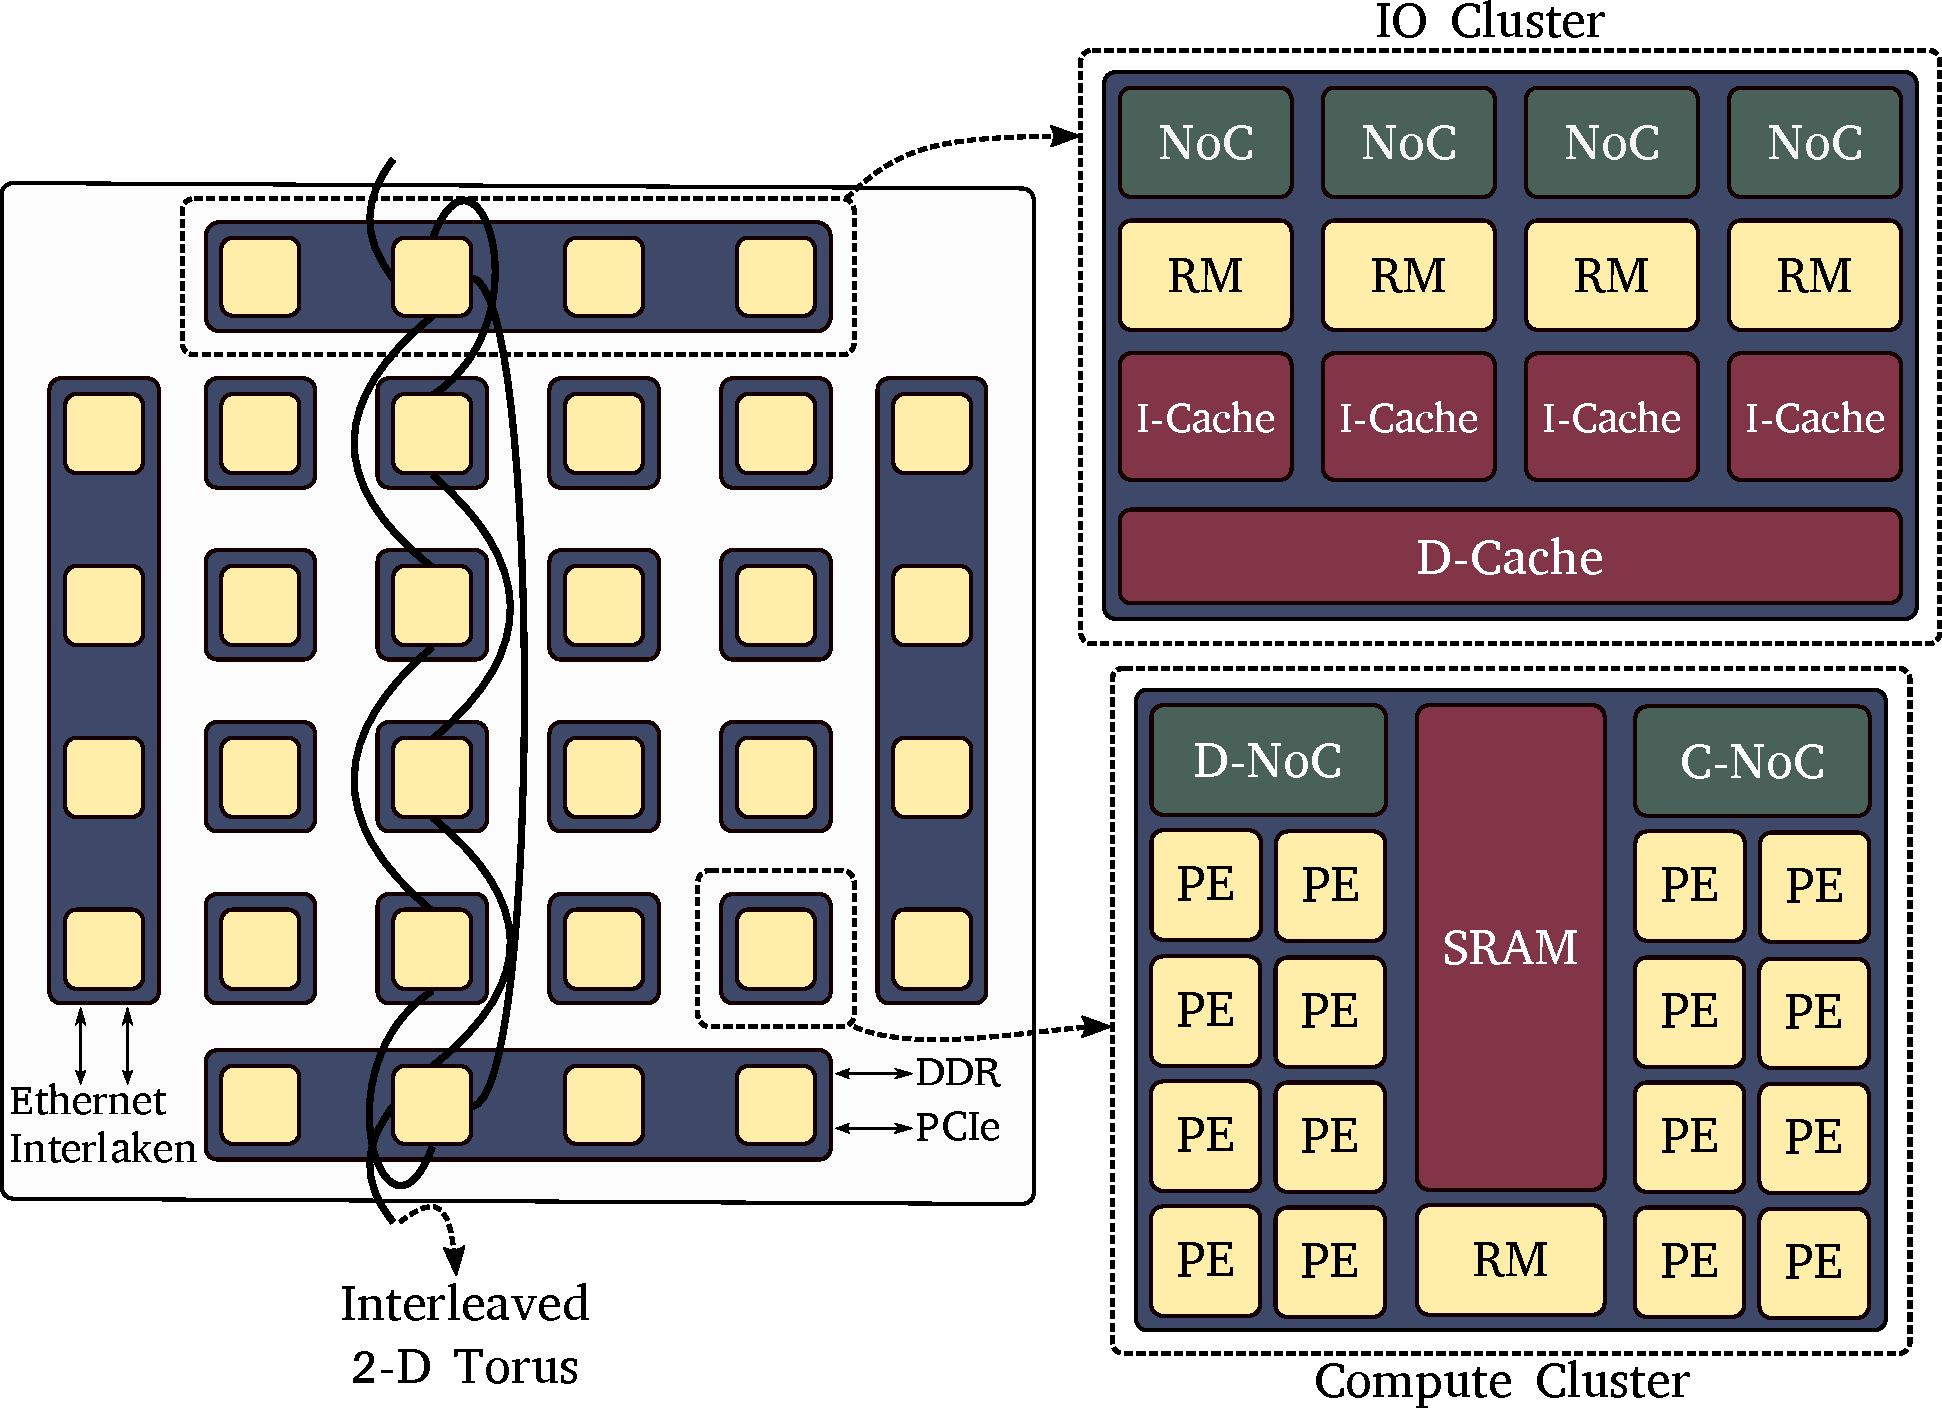
\includegraphics[width=0.50\linewidth]{images/arch-mppa.pdf}
        \label{fig:mppa}
      \end{figure}
    \end{frame}

% Força todas referências a aparecerem
\nocite{*}

\section{Referências}
  \begin{frame}{Referências Bibliográficas}
    \begin{thebibliography}{10}
      \bibitem{Souto et. al} João V. Souto and Pedro H. Penna and Castro, Márcio.
      \textcolor{blue}{\em An Inter Cluster Communication Facility for Lightweight Manycore
        Processors in the Nanvix OS}.
      {UFSC, $2019$}.

      \medskip

      \bibitem{MPI Forum} Message Passing Interface Forum. \textcolor{blue}{\em MPI: A Message
        Passing Interface Standard Version 3.1} {HLRS, 2015}

      \medskip

      \bibitem{Penna et. al} Pedro H. Penna and Souto, João and Lima, Davidson F. and
        Castro, Márcio and Broquedis, François and Freitas, Henrique H. and Mehaut, Jean François.
        \textcolor{blue}{\em On the Performance and Isolation of Asymmetric Microkernel Design for
        Lightweight Manycores}. {HAL-Archive-Ouvertes, $2019$}.
    \end{thebibliography}
  \end{frame}

%%%%%%%%%%%%%%%%%%%%%%%%%%%%
% Finalização
%%%%%%%%%%%%%%%%%%%%%%%%%%%%

% Thanks frame
\begin{frame}{Finalização}
  \begin{center}
    \Huge{Dúvidas?} \\
    \Huge{Obrigado!}
  \end{center}
\end{frame}

\end{document}
